\documentclass[11pt]{article}

\usepackage{report}

\usepackage[utf8]{inputenc} % allow utf-8 input
\usepackage[T1]{fontenc}    % use 8-bit T1 fonts
\usepackage[colorlinks=true, linkcolor=black, citecolor=blue, urlcolor=blue]{hyperref}       % hyperlinks
\usepackage{url}            % simple URL typesetting
\usepackage{booktabs}       % professional-quality tables
\usepackage{amsfonts}       % blackboard math symbols
\usepackage{nicefrac}       % compact symbols for 1/2, etc.
\usepackage{microtype}      % microtypography
\usepackage{lipsum}		% Can be removed after putting your text content
\usepackage{graphicx}
\graphicspath{ {./images/} }
\usepackage{natbib}
\usepackage{doi}
\setcitestyle{aysep={,}}
\usepackage{array}

\usepackage{listings}
\usepackage{xcolor}
\definecolor{codegreen}{rgb}{0,0.6,0}
\definecolor{codegray}{rgb}{0.5,0.5,0.5}
\definecolor{codeorange}{rgb}{1,0.49,0}
\definecolor{backcolour}{rgb}{0.95,0.95,0.96}

\lstdefinestyle{mystyle}{
    backgroundcolor=\color{backcolour},   
    commentstyle=\color{codegray},
    keywordstyle=\color{codeorange},
    numberstyle=\tiny\color{codegray},
    stringstyle=\color{codegreen},
    basicstyle=\ttfamily\footnotesize,
    breakatwhitespace=false,         
    breaklines=true,                 
    captionpos=b,                    
    keepspaces=true,                 
    numbers=left,                    
    numbersep=5pt,                  
    showspaces=false,                
    showstringspaces=false,
    showtabs=false,                  
    tabsize=2,
    xleftmargin=10pt,
}

\lstset{style=mystyle}

\title{CT255 - Next Gen Technologies II}

\author{Andrew Hayes\\
\AND
Student ID: 21321503\\
\AND
\AND
\AND
\AND
	2BCT\\
\AND
    University of Galway\\
}

% Uncomment to remove the date
\date{February 2022}

% Uncomment to override  the `A preprint' in the header
\renewcommand{\headeright}{2D Games Programming in Java}
\renewcommand{\undertitle}{2D Games Programming in Java}
\renewcommand{\shorttitle}{}

%%% Add PDF metadata to help others organize their library
%%% Once the PDF is generated, you can check the metadata with
%%% $ pdfinfo template.pdf
% \hypersetup{
% pdftitle={A template for the arxiv style},
% pdfsubject={q-bio.NC, q-bio.QM},
% pdfauthor={David S.~Hippocampus, Elias D.~Striatum},
% pdfkeywords={First keyword, Second keyword, More},
% }

\begin{document}
\maketitle

\newpage
\tableofcontents
\thispagestyle{empty}


\newpage
\setcounter{page}{1}
\section{Lecture 1}
\subsection{2D Co-Ordinate System}
The \textbf{JFrame} class will provide a Window with associated graphics canvas \& a pixel-based
co-ordinate system with the origin at (0,0) on the top \textbf(left). 
A JFrame is a top-level window with a title \& a border. 
To have access to JFrame and associated methods:
\\
\verb|import java.awt.*;|   \\
\verb|import javax.swing.*;|


The top 50 pixels or so are hidden by the window's title bar (depending on the operating system).

\subsection{Basic Graphics in Java}
2D graphics can be drawn using the \verb|Graphics| class. 
This provides methods for drawing ``primitives'' (lines, circles, boxes) and also images (.jpg, .png, etc.). 

The \verb|paint()| method of the \verb|JFrame| class is automatically invoked whenever it needs to be 
painted (system-invoked). 
Otherwise, you can force painting to happen via \verb|repaint()| if you need to repaint when the OS
doesn't think that it's needed.

\begin{lstlisting}[language=Java]
    public void paint (Graphics g) {
        // use the "g" object to draw graphics
    }
\end{lstlisting}

\subsection{Drawing Text using Methods of the Graphics Class}
\begin{lstlisting}[language=Java]
    public void paint (Graphics g) {
        Font f = new Font("Times", Font.PLAIN, 24);
        g.setFont(f);
        Color c = Color.BLACK;
        g.setColor(c);
        g.drawString("Pacman!", 20, 60);
    }
\end{lstlisting}.

This should be added as a method of the application class.

\section{Lecture 2}         
\subsection{Animation with Threads}

\textbf{Animation} is the changing of grahics over time, e.g., moving a spaceship across the screen, changing its position by 
one pixel every 0.02 seconds. 

One of the best ways to do periodic execution of code is to use \textbf{threads}. 
Threads allow multiple taks to run independently/concurrently within a program. 
Essentially, this means that we spawn a separate execution ``branch'' that operates independently of our program's main flow of control. 
For example, the new thread could repeatedly sleep for 20ms, then carry out an animation, and call \verb|this.repaint()| on the application. 

\subsubsection{Implementing Threads in Java} 
Your application class should implement the \verb|Runnable| interface, i.e.:
\begin{lstlisting}[language=Java]
public class MyApplication extends JFrame implements Runnable {
}
\end{lstlisting}

Your application now \textbf{must} provide an implementation for the \verb|run()| method, which is executed when a thread is started, serving as its ``main'' function, i.e.:
\begin{lstlisting}[language=Java]
public void run(){
}
\end{lstlisting}

To create \& start a new thread running from your application class:
\begin{lstlisting}[language=Java]
Thread t = new Thread(this);
t.start();
\end{lstlisting}

The typical actions of an animation thread are as follows:
\begin{enumerate}
    \item   Sleep for (say) 20ms using \verb|Thread.sleep(20);|. Note that you will be \textbf{required} to handle \verb|InterruptedException|. 
    \item   Carry out movement of game objects. 
    \item   Call \verb|this.repaint();| which (indirectly) invokes our \verb|paint(Graphics g)| method. 
    \item   Go back to Step 1. 
\end{enumerate} 

\subsubsection{Threads Test}
\begin{lstlisting}[language=Java]
import java.awt.*;
import javax.swing.*; 

public class ThreadsTest implements Runnable {
    public ThreadsTest() {
        Thread t = new Thread(this); 
        t.start(); 
    }

    public void run() {
        System.out.println("Thread started");

        for (int i = 0; i < 15; i++) {
            System.out.println("Loop " + i + "Start"); 
            try {
                Thread.sleep(500);
            } catch (InterruptedException e) {
                // TODO Auto-generated catch block 
                e.printStackTrace(); 
            } 
            System.out.println("Loop " + i + " end"); 
        }
        System.out.println("Thread ended"); 
    }

    public static void main(String[] args) {
        ThreadsTest tt = new ThreadsTest(); 
    }
}
\end{lstlisting}

\subsection{Game Object Classes}
Games typically have \textbf{game object classes} (spaceships, alines, cars, bullets, etc.). 
Numerous instances of each may exist at runtime. 
This class encapsulates the data (position, colour, etc.) and code (move, draw, die, etc.) associated with the game object.

Typically, we store these instances in a data structure such as an array, so that during our animation \& painting phases we can iterated through them all and invoke the \verb|animate()| \& \verb|paint()| methods on each instance. 

\section{Lecture 03}
\subsection{Handling Keyboard Input}
In GUI-based languages such as Java (with AWT), the mouse \& keyboard are handled as ``\textbf{events}''. 
These events may happen at any time. 
Events are queued as they happen and are dealt with at the next free, idle time. 
AWT handles events coming from the OS by dispatching them to \textit{listeners} registered to those events. 

To handle keyboard input:
\begin{enumerate}
    \item   Make a class that implements \verb|KeyListener|. Make sure that you have an instance of this class. 
    \item   Add this instance as a key listener attached to the \verb|JFrame| that receives the messages from the OS. 
            The simplest way is to make your JFrame-derived class handle the events it receives itself. 
\end{enumerate} 

\begin{lstlisting}[language=Java]
import java.awt.*;
import java.awt.event.*;
import javax.swing.*; 

public class MyApplication extends JFrame implements KeyListener {
    public MyApplication() {
        // send keyboard events arriving into this JFrame to its own event handlers. 
        addKeyListener(this);
    }

    // 3 keyboard event handler functions 
    public void keyPressed(KeyEvent e) {
    }
    public void keyReleased(Event e) {
    }
    public void keyTyped(KeyEvent e) {
    }
}
\end{lstlisting}

Notes:
\begin{itemize}
    \item   The \verb|KeyEvent| parameter \verb|e| provides the ``virtual keycode'' of the key that has triggered the event, and constants are defined to match these values, e.g., \verb|KeyEvent.VK_Q| or \verb|KeyEvent.VK_ENTER|. 
    \item   To get the keycode, use \verb|e.getKeyCode()|.
    \item   For our game applications, our application class will implement both \verb|KeyListener| \& \verb|Runnable|. 
    \item   Note the extra import: \verb|import java.awt.event.*;|. 
\end{itemize}

\subsection{Loading \& Displaying Raster Images}
The constructor of the \verb|ImageIcon| class (defined in \verb|javax.swing| loads an image from disk (\verb|.jpg|. \verb|.gif|, or \verb|.png|) and returns it as a new instance of the \verb|ImageIcon| class. 

The \verb|getImage()| method of this \verb|ImageIcon| object gives you a useable \verb|Image| class object, which can be displayed in your \verb|paint()| method by the \verb|Graphics| class. 

\begin{lstlisting}[language=Java] 
import java.awt.*;
import javax.swing.*;

public class DisplayRasterImage extends JFrame {
    // member data
    private static String workingDirectory; 
    private Image alienImage; 

    // constructor 
    public DisplayRasterImage() {
        // set ip JFrame 
        setBounds(100, 100, 300, 300); 
        setVisible(true); 

        // load image from disk. Make sure you have the path right! 
        ImageIcon icon = new ImageIcon(workingDirectory + "/alien_ship_1.png");
        alienImage = icon.getImage(); 

        repaint();
    }

    // application's paint method (may first happen *before* image is finished loading, hence repaint() above 
    public void paint(Graphics g) {
        // draw a black rectangle on the whole canvas 
        g.setColor(Color.BLACK);
        g.fillRect(0,0,300,300);

        // display the image (final argument is an "ImageObserver" object)
        g.drawImage(alienImage, 150, 150, null); 
    }

    // application entry point 
    public static void main(String[] args) {
        workingDirectory = System.getProperty("user.dir");
        System.out.println("workingDirectory = " + workingDirectory); 
        DisplayRasterImage d = new DisplayRasterImage(); 

    }
}
\end{lstlisting} 

\section{Lecture 04 - Screen Flicker} 
Screen flicker is caused by software redrawing a screen out of sync with the screen being refreshed by the graphics hardware, 
resulting in a half-drawn image occasionally being displayed. 

The solution to screen flicker is to use \textbf{double buffering}. 
Double buffering involves first rendering all graphics to an offscreen \textit{memory buffer}.  
Then, when finished drawing a frame of animation, flip the offscreen buffer onscreen furing the ``vertical sync'' period. 

\verb|java.awt| provides a \verb|BufferStrategy| class that applies the best approach based off the capabilities of the 
computer on which the software is running.

\subsection{Implementing Double Buffering} 
\begin{enumerate}
    \item   \verb|import java.awt.image.*;| 
    \item   Add a new member variable to the Application class: \verb|private BufferStrategy strategy;| 
    \item   In the Application class's constructor method: 
            \begin{lstlisting}[language=Java] 
createBufferStrategy(2); 
strategy = getBufferStrategy(); \end{lstlisting}
            Note that this code should be executed \textbf{after} the JFrame has been displayed, i.e. after \verb|setBounds()| 
            \& \verb|setVisible()|. 
    \item   At the start of the \verb|paint(Graphics g)| method, include \verb|g = strategy.getDrawGraphics();| to redirect our 
            drawing calls to the offscreen buffer. 
    \item   At the end of the \verb|paint(Graphics g)| method, include \verb|strategy.show();| to indicate that we want to flip 
            the buffers.
\end{enumerate}

\section{Lecture 05 - Finishing Space Invaders} 
\subsection{Animated 2D Sprites}
To animate a 2D sprite, we can simply load two or more images and alternate or cycle between them. 
For our game, switching image once per second (i.e., every 50$\textsuperscript{th}$ redraw is about right). 

E.g., use this in a modified \verb|Sprite2D| class.
\begin{lstlisting}[language=Java]
public void paint(Graphics g) {
    framesDrawn++;
    if (framesDrawn % 100 < 50) {
        g.drawImage(myImage, (int) x, (int) y, null); 
    } 
    else {
        g.drawImage(myImage2, (int) x, (int) y, null); 
    }
}
\end{lstlisting}

\subsection{Collision Detection} 
To detect collisions, we cna simply check for overlapping rectangles.
\begin{lstlisting}[language=Java]
if ( ((x1<x2 && x1+w1>x2) ||(x2<x1 && x2+w2>x1) ) && ( (y1<y2 && y1+h1>y2 ) || (y2<y1 && y2 + h2>y1) ) ) 
\end{lstlisting}

\subsection{Game States} 
Games normally have at least two high-level ``states'', i.e., is the game in progress or are we currently displaying 
a menu before the game starts (or after it finishes)? 
To do this, we can simply add a boolean member to the application class: \verb|isGameInProgress|. 
Depending on the value of this, we can handle various things differently:
\begin{itemize}
    \item   Keypresses. 
    \item   The \verb|paint()| method. 
    \item   The thread's game loop. 
\end{itemize} 

\section{Lecture 06 - Conway's Game of Life}
\subsection{Mouse Events}
Mouse events notify when the user uses the mouse (or similar input device) to interact with a component.
Mouse events occur when the pointer enters or exits a component's onscreen area and when the user presses or releases one of the mouse buttons. 

Additional events such as mouse movement \& the mouse wheel can be handled by implementing the \verb|MouseMotionListener| 
and \verb|MouseWheelListener| interfaces.
\begin{enumerate}
    \item   Have your class implement \verb|MouseListener|. 
    \item   Add \verb|addMouseListener(this);| to the clas constructor. 
    \item   Implement the methods below: 
        \begin{lstlisting}[language=Java]
// mouse events which must be implemented for MouseListener 
public void  mousePressed(MouseEvent e) { }
public void mouseReleased(MouseEvent e) { }
public void  mouseEntered(MouseEvent e) { }
public void   mouseExited(MouseEvent e) { }
public void  mouseClicked(MouseEvent e) { }
\end{lstlisting}
\end{enumerate}

\subsection{Conway's Game of Life: Rules}
\verb|private boolean gameState[][][] new boolean[40][40][2];|

\begin{enumerate}
    \item   Any live cell with fewer than two live neighbours dies, as if caused by under-population.
    \item   Any live cell with two or three live neighbours lives on to the next generation.
    \item   Any live cell with more than three live neighbours dies, as if by overcrowding. 
    \item   Any dead cell with exactly three live neighbours becomes a live cell, as if by reproduction.
\end{enumerate}

Each generation (iteration) of the game is created by applying the above rules simultaneously to every cell in its 
preceding generation: births \& deaths occur simultaneously.
To implement this properly, we will need to have two separate game states in memory:
\begin{itemize}
    \item   One is the ``front buffer'' that we are currently displaying, and which we are checking the above rules on. 
    \item   The other is the ``back buffer'' that we're applying the results of the rules to.
    \item   The ``back buffer'' will be switched to the ``front'' after applying the rules to every cell.
\end{itemize}

We will check the eight neighbours of each cell as follows:
\begin{lstlisting}[language=java]
for (int x=0;x<40;x++) {
    for (int y=0;y<40;y++) {
        // count the live neighbours of cell [x][y][0]
        for (int xx=-1;xx<=1;xx++) {
            for (int yy=-1;yy<=1;yy++) {
                if (xx!=0 || yy!=0) {
                    // check cell [x+xx][y+yy][0]
                    // but.. what if x+xx==-1, etc. ?
                }
            }
        }
    }      
}
\end{lstlisting}

Note that we need to define the neighbours for cells at the edges of the map. 
The usual procedure is to ``wrap around'' to the opposite side.

\subsection{Another Example of a Cellular Automata Algorithm in Use}
The image below is of an algorithmically-generated cave-like structure, for use in a 2D computer game.
Each of the cells, laid out in a 60x30 grid, either has a wall (denoted by \verb|#|) or a floor (denoted by \verb|.|).

The cellular automata algorithm which generated this output uses the following steps:
\begin{itemize}
    \item   For each cell, randomly define it as: wall (60\% chance) or floor (40\% chance). 
    \item   Perform the following procedure four times: Calculate the number of wall neighbours for each cell, and 
            define each cell which has at least 5 neighbouring wall cells, as a wall cell itself.
            Otherwise (i.e., if it has less than 5 wall neighbours), define it as a floor cell.
\end{itemize}

\begin{center}
    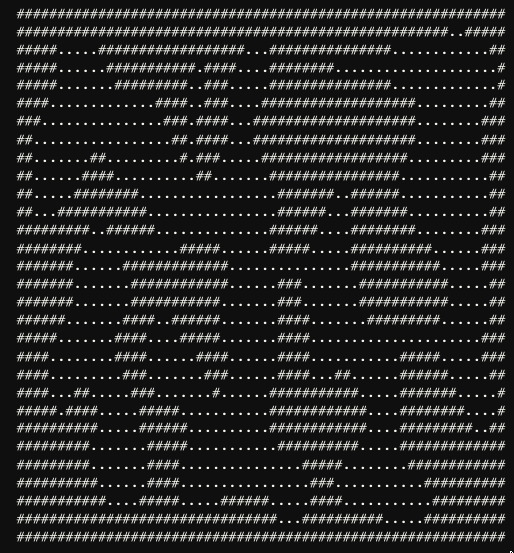
\includegraphics[width=0.6\textwidth]{cave.png}
\end{center}

\section{Week 8}
\subsection{Reading from Text Files}
The \verb|java.io| provides file handling classes:
\begin{itemize}
    \item   \verb|FileReader| to read from a text file. 
    \item   \verb|BufferedFileReader| to read from a text file more efficiently (reads larger blocks \& buffers/caches them). 
            \begin{itemize}
                \item   \textit{Exception handling is required.}
                \item   Uses the \verb|FileReader| class constructor to open a file.
                \item   Uses the \verb|readLine()| method to read a line of text (which returns a \verb|String|).
                \item   Uses the \verb|close()| method to close the file.
            \end{itemize}
\end{itemize}

Sample code that reads just one line from the file (stopping at the end of the file or when a carriage return is encountered): 
\begin{lstlisting}[language=java]
String filename = "C:\\Users\\Sam\\Desktop\\lifegame.txt";
String textinput = null;
try {
    BufferedReader reader = new BufferedReader(new FileReader(filename));
    textinput = reader.readLine();
    reader.close();
} 
catch (IOException e) { }
\end{lstlisting}
    
Sample code that reads all the carriage return-separated lines from a file: 
\begin{lstlisting}[language=java]
String line=null;
String filename = "C:\\Users\\Sam\\Desktop\\lifegame.txt";
try {
    BufferedReader reader = new BufferedReader(new FileReader(filename));
    do {
        try {
            line = reader.readLine();
            // do something with String here!
        } catch (IOException e) { }
    }
    while (line != null);

    reader.close();

} catch (IOException e) { }
\end{lstlisting}

\subsection{Writing to Text Files}
Use the \verb|FileWriter| \& \verb|BufferedWriter| classes:

\verb|BufferedWriter|:
\begin{enumerate}
    \item   Use the \verb|FileWriter| class constructor to open a file. 
    \item   Use the \verb|write(String s)| method to write a line to the file (with a CR appended automatically).
    \item   Use the \verb|close()| method to close the file.
\end{enumerate}

E.g., to write a single String to a file:
\begin{lstlisting}[language=java]
String filename = "C:\\Users\\Sam\\Desktop\\lifegame.txt";
try {
    BufferedWriter writer = new BufferedWriter(new FileWriter(filename));
    writer.write(outputtext);
    writer.close();
} 
catch (IOException e) { }
\end{lstlisting}

\subsection{Handling Mouse Motion Events} 
In addition to mouse button events, we can also receive mouse \textit{movement} events. 
Have the class implement the \verb|MouseMotionListener| interface as well as \verb|MouseListener|. 
In the application class constructor have: \verb|addMouseMotionListener(this);|. 
Add these methods (receives the same data as the mouse events we have already seeen): 
\begin{lstlisting}[language=Java] 
public void mouseMoved(MouseEvent e)
public void mouseDragged(MouseEvent e)
\end{lstlisting}


This is useful for making it less tedious to create a new initial game set-up.

\section{A* Pathfinding}
The fundamental operations of the \textbf{A*} algorithm is to traverse a map by exploring promising positions (nodes) beginning at a starting location, witht the goal of finding the best route to a target location. 

Each node has four attributes, other than its position on the map:
\begin{itemize}
    \item   $g$ is the cost of getting from the starting node to this node. 
    \item   $h$ is the heuristic (estimated) cost of getting from this node to the target node. 
            $h$ is a best guess, since the algorithm does not yet know the actual cost.
    \item   $f$ is the sum of $g$ \& $h$, and is the algorithm;s best current estimate as to the total cost of travelling from the starting location to the target location via this node.
    \item   \textit{parent} is the identity of the node which connected to this node along a potential solution path.
\end{itemize}

The algorithm maintains two lists of nodes: the \textbf{open} list \& the \textbf{closed} list. 
\begin{itemize}
    \item   The open list consists of nodes to which the algorithm has already found a route, i.e. one of its connected neighbours has been evaluated (\textit{expanded}) but which have not yet themselves been expanded.
    \item   The closed list consists of nodes that have been expanded and which therefore should not be re-visited.
\end{itemize}

Progress is made by identifying the most promising node in the open list, i.e., the one with the lowest $f$ value, and expanging it by adding each of its connected neighbours to the open list, unless they are 
already closed.
As nodes are expanded, they are moved to the closed list. 
As nodes are added to the open list, their $f$, $g$, $h$, \& \textit{parent} values are recorded.
The $g$ value of a node is, of course, equal to the $g$ value of its parent plus the cost of moving from the parent to the node itself.

\begin{center}
    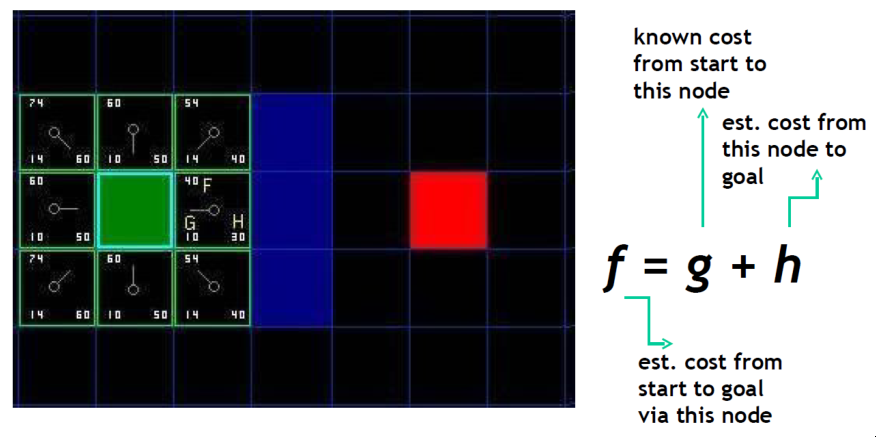
\includegraphics[width=0.7\textwidth]{astar.png}
\end{center}

\subsection{Implementing A* Pathfinding}


\bibliographystyle{unsrtnat}
\bibliography{references}
\end{document}

